\skriptsection{Linear Discriminant Functions}{215}
  Assume, that the \emph{form} of the discriminant functions are known instead of the
  distributions. The problem of finding a linear discriminant function can be formulated as a problem
  of \emph{minimizing a criterion function}, e.g. the sample risk or the training error.
  But a small training error doesn't guarantee a small test error.
  

  \skriptsubsection{Linear Discriminant Functions and Decision Surfaces}{216}
    \skriptsubsubsection{Two-Category Case}{216}
      The same forms as in \ref{sec:bayes_discriminant_function} (page \pageref{sec:bayes_discriminant_function}) 
      of this summary are used here:
      $$g(\bm x) = \bm w ^T \bm x + w_0$$
      Decide $\omega_1$ when $g(\bm x) > 0$ and $\omega_2$ when $g(\bm x) < 0$. $g(\bm x) = 0$ is
      the decision surface, it is a hyperplane in the linear case and it is normal to the weights 
      $\bm w$.
      
    \begin{multicols}{2}
	    \skriptsubsubsection{Multicategory Case}{218}
		There exist several possibility to create multicategory classifier with $c$ classes.
		We could use $c$ linear discriminant functions to separate points belonging 
		to $\omega_i$ and those not belonging to $\omega_i$.
		Another possibility would be to create $c(c-1)/2$ discriminants, one for each pair of classes.
		Both aproaches lead to undefined ambiguous regions.
	
		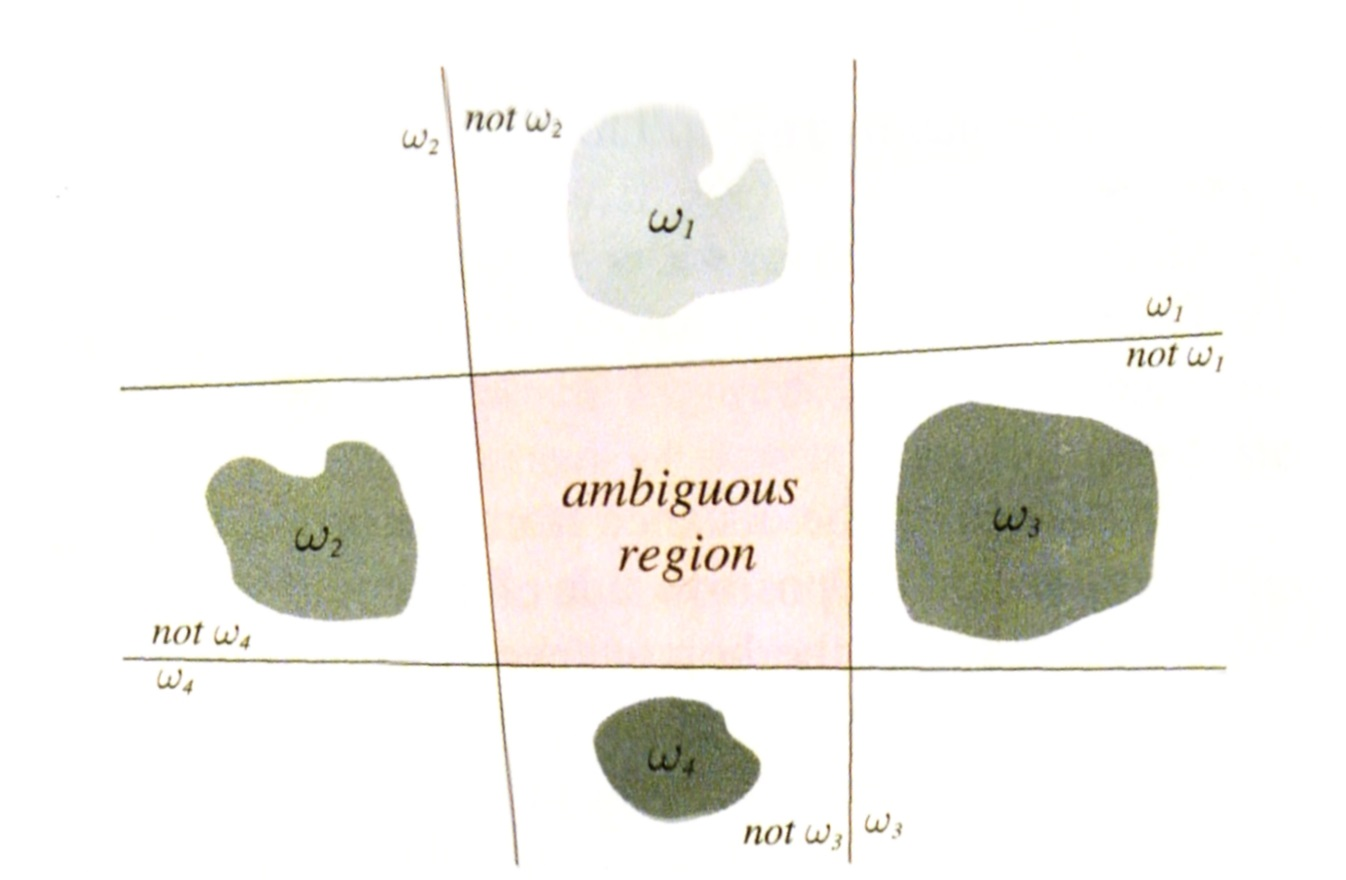
\includegraphics[width=0.5\linewidth]{images/onevsall.jpg}
		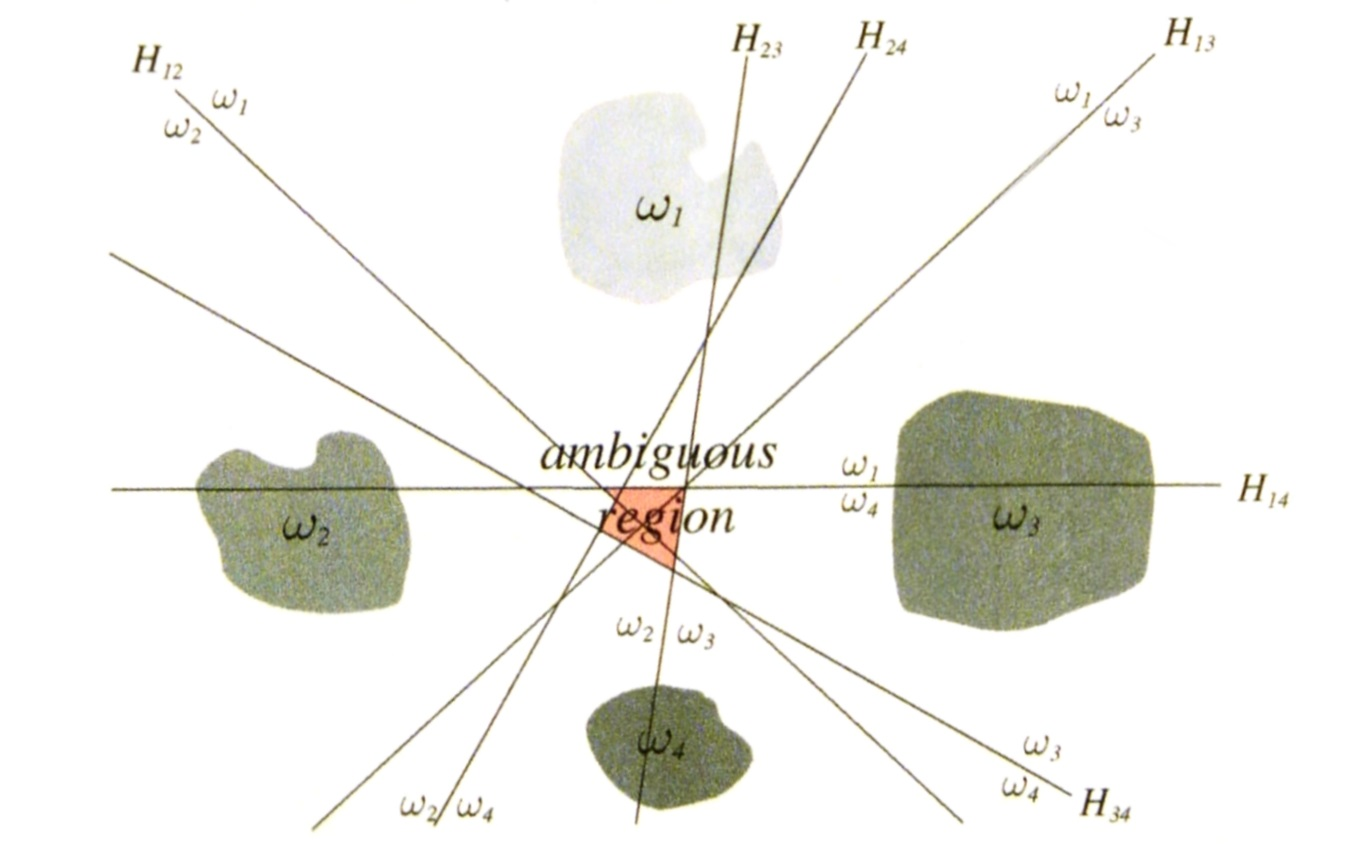
\includegraphics[width=0.5\linewidth]{images/onevsone.jpg}
    \end{multicols}
    
    By defining $c$ linear discriminant functions
    \begin{equation*}
	    g_i(\bfx) = \mathbf{w}_i^t\bfx + w_{i0} \quad i=1,\ldots,c
    \end{equation*}
	we can assign $\bfx$ to $\omega_i$ if $g_i(\bfx) > g_j(\bfx)$ for all $j \neq i$.
	This classifier is called a \emph{linear machine}.
      
  
  \skriptsubsection{Generalized Linear Discriminant Functions}{219}
  \label{sec:generalized_linear_discriminant_function}
  
  \begin{multicols}{2}
	  \subsubsection{Quadratic Discriminant Function}
	      By multiplying features with itself, ``new'' features can be created and possibly improve the classification
	      results. This results in the quadratic discriminant function
	      
	      \begin{equation*}
		      g(\bm x) = w_0 + \sum\limits_{i=1}^d w_i x_i + \sum\limits_{i=1}^d \sum\limits_{i=1}^d w_{ij} \underbrace{x_i x_j}_{\text{new feature}}
	      \end{equation*}
	      
	      and can produce more complicated separating surfaces, because the problem will be mapped in a more dimensional space.
	      The data itself uses not more dimensions. E.g. The data of an one dimension problem stays on one line. \\
	      
      	 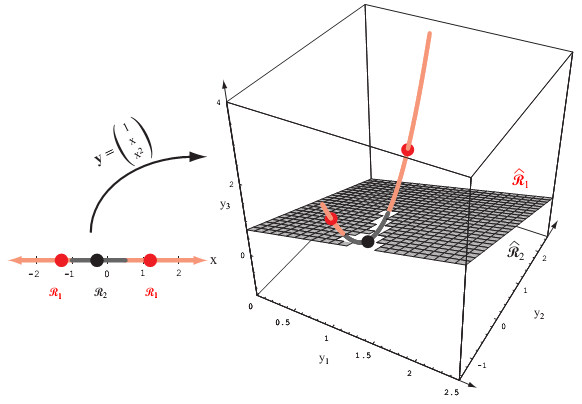
\includegraphics[width=6cm]{./images/map1DTo2D.png} \\
       	 Feature mapping from one dimension into 2D with $x^2$ \\
       \columnbreak	 
   	   \subsubsection{Generalized Linear Discriminant Functions}
   	     By continuing this approach, polynomial discriminant function or generalized linear discriminant 
   	     functions are evolving: 
   	     $$g(\bm x) = \sum\limits_{i=1}^{\hat d} a_i y_i(\bm x) = \bm a^T \bm y$$
   	     $\bm a$ is a 
   	     $\hat d$-dimensional weight vector and the $\hat d$ functions $y_i(\bm x)$ ($\varphi$-functions 
   	     or augmented features) are arbitrary functions of $\bm x$ and \textbf{don't have to be linear}.
   	     Therefore, the discriminant functions are linear in $\bm y$ but not in $\bm x$.\\
   	     The disadvantage is a high computational complexity with high dimensions and that much 
   	     \textbf{more trainings data} are needed to avoid overfitting.
   	     
    \subsubsection{Augmented Feature Vector}
      To include the offset $w_0$ of the discriminant function $g(\bm x) = w_0 + w_1 x_1 + w_2 x_2 + \ldots + w_n x_d$ into the weight vector $\bm w$ 
      a one is added to the feature vector  $\bm y = [1, x_1, x_2, \ldots, x_n]^T = [1, \bm x]^T$.
      This vector is called \emph{augmented feature vector} and the resulting weight vector $\bm a = [w_0, w_1, w_2, \ldots w_d]^T = [w_0, \bm w]^T$  \emph{augmented
      weight vector}.
      The discriminant function can then be written as $g(x) = \mathbf{a}^T \mathbf{y}$.
      The decision boundary can now be interpreted as a hyperplane going through $[0,\ldots,0]$ and 
      all data lies on the level at $y_0=1$.
      The separation plane equation is then $\mathbf{a}^T \mathbf{y} = 0$ with $\mathbf{y} = \begin{bmatrix}1 & x_1& x_2\end{bmatrix} \Rightarrow x_1=-\frac{a_0 + a_2\cdot x_2}{a_1}$
  \end{multicols}      


   
  \subsection{Two-Category Linearly Separable Case}

    If a linear weight vector exists that classifies all samples correctly, then the samples
    are said to be linearly separable.

    \begin{minipage}{11cm}
    
    \skriptsubsubsection{Normalization / Margin}{223}
    In the separable case, the vector product of every training sample of class $\omega_1$ with the solution
    vector $\bm a$ is positive, and with the class $\omega_2$ is negative.\\
    For easier handling of the training data, all samples labeled $\omega_2$ are replaced by their negatives.
    Now the vector product of the solution vector $\bm a$ with \emph{every} training sample will have to be positive 
    $\bm a^T \bm y_i  > 0$ \\
    
    The separating vector usually doesn't have one single solution but it can lie in a solution
    region. Furthermore, $\bm a$ should not lie on the boundary and therefore a margin $b$
    can be introduced. \\
        
    A normalized augmented feature for a 2-dimensional problem can then look like:
    $\bm y = \begin{bmatrix}
      1 & 1 & 2\\
      1 & 2 & 0\\
      -1 & -3 & -1\\
      -1 & -2 & -3
    \end{bmatrix}$.
    \end{minipage}
    \hspace{5mm}
    \begin{minipage}{7cm}
    	 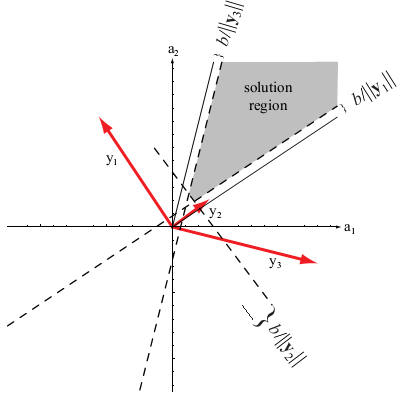
\includegraphics[width=7cm]{./images/solutionRegionWithMargin.png}
    	 Solution region of a ``normalized" vector with margin $b$
 	\end{minipage}
    
    \skriptsubsubsection{Basic Gradient Descent}{224}
      The basic approach to find a solution vector is the method of steepest descent. The aim is to
      minimize a defined criterion function $J_a$ and it is solved iteratively with every step calculating
      $$\bm a (1) \text{ arbitrary}$$
      $$\bm a (k+1) =  \bm a(k) - \eta(k) \nabla J(\bm a(k))$$
      with $\eta > 0$ being the step size or learning rate. When $\eta$ is too small, convergence is
      needlessly slow, with $\eta$ being large the correction can overshoot and even diverge.\\
      The \textbf{optimal step size} can be calculated with:
      $\eta(k)= \frac{\|\bm{\nabla J}\|^2}{\bm{\nabla J^T  H \nabla J}}$ where $\bm H$ is the Hessian matrix
       (matrix of second partial derivatives $\partial^2 J / \partial a_i \partial a_j$, see Newton's Algorithm).
      Calculating the Hessian matrix in every step is normally too expensive so that the optimal solution is used very seldom.

    \skriptsubsubsection{Newton's Algorithm}{226}
      The Newton method is not used widely due to the fact that a matrix has to be inverted on every
      step:
      $$\bm a(k+1) = \bm a(k) - \bm H^{-1} \bm \nabla \bm J \text{ with Hessian matrix } \bm H = \begin{bmatrix}
      \frac{\delta^2 f}{\delta x_1^2} & \ldots & \frac{\delta^2 f}{\delta x_1 \delta x_n}\\
      \vdots & \ddots & \vdots \\
      \frac{\delta^2 f}{\delta x_n \delta x_1} & \ldots & \frac{\delta^2 f}{\delta x_n^2}\\
      \end{bmatrix}$$
      This is a simplification of the optimum step size from the section above.
  
  \skriptsubsubsection{Minimizing the Perceptron Criterion Function}{227}
  \begin{minipage}{12cm}
    The problem is to construct a criterion function for solving the linear inequalities $\bm a^T \bm y > 0$. 
    A criteria function which just counts the misclassified sample would be constant at the most position. 
    Therefore the steepest descent would not work. \\
    
    A better idea is the \textbf{Perceptron Criterion Function}
    $\bm J_p(\bm a) = \sum\limits_{\bm y \in \mathcal{Y}_k} (-\bm a^T \bm y)$  with $\mathcal{Y}$ as the set
    of misclassified samples by the current weight vector $\bm a$.\\
    The gradient is $\bm {\nabla J}_p = \sum\limits_{\bm y\in \mathcal{Y}_k} -\bm y$
    which leads to the update rule 
    \begin{equation*}
        \bm a(k+1) = \bm a(k) + \eta(k) \sum\limits_{\bm y\in \mathcal{Y}_k} \bm y
    \end{equation*}
       
   	\end{minipage}
    \hspace{8mm} 
    \begin{minipage}{6cm}
    	 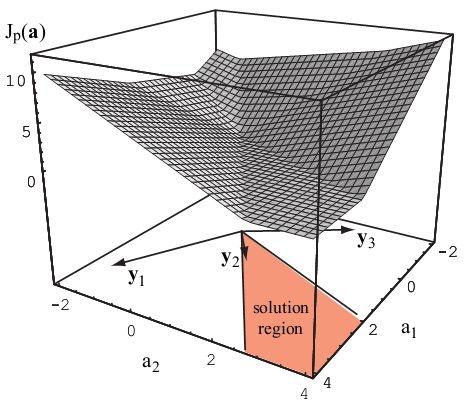
\includegraphics[width=6cm]{./images/perceptron.png}
    \end{minipage} \\
    
    \begin{multicols}{3}
        \skriptsubsubsubsection{Batch Perceptron}{228}\\
        The batch perceptron algorithm yields in a solution for linearly separable problems. 
        It sums up all misclassified samples and then performs a weight update (batch). 
        This has to be done until all of the samples will be classified correctly.  
    \vfill
    \columnbreak
        \skriptsubsubsubsection{Fixed-Increment Single-Sample Perceptron}{230}\\
        The fixed-increment single-sample perceptron algorithm changes the weight vector
        with every (misclassified) sample and therefore saves many computations.
    \vfill
    \columnbreak
        \skriptsubsubsubsection{Variable-Increment Perceptron with Margin}{233}\\
        Additionally, the increment factor $\eta(k)$ can be variable. E.g. $\eta(k)=1/k$. For better 
        generalization, a margin $b$ can be added as shown in algorithm 5.  
    \end{multicols}

    
    \skriptsubsubsection{Relaxation Procedures}{235}
    \begin{minipage}{12cm}
    The \emph{descent algorithm} uses a square in the criterion function:
	$\bm J_q(\bm a) = \sum\limits_{\bm y \in \mathcal{Y}_k} (\bm a^T \bm y)^2$ with $\mathcal{Y}$ as the set
    of misclassified samples.\\
    
  	Because the gradient is continuous, the criterion function $\bm J_q$ is smoother. The problem is that the algorithm is too smooth at the border and 
  	the algorithm can converge to the border or worse to $\bm a=0$. 
  	Another problem is that $\bm J_q$ is dominated by long training samples. \\
  	
  	A criterion function which solves both problems is: 
  	$\bm J_r(\bm a) = \frac{1}{2} \sum\limits_{\bm y \in \mathcal{Y}_k} \frac{(\bm a^T \bm y - b)^2}{\|\bm y\|^2}$
  	where $b$ is a new margin and $\mathcal{Y}(\bm a)$ is the set of samples for which $\bm a^T \bm y \leq b$. $J_r$ is never 
  	negative and only zero when the whole set has been classified correctly inside margin.
  	
  	This leads to the update rule
  	$\mathbf{a}(k+1) = \mathbf{a}(k) + \eta(k)\sum_{\mathbf{y}\in\mathcal{Y}}\frac{b-\mathbf{a}^t\mathbf{y}}{||\mathbf{y}||^2}\mathbf{y}$
  	and the single-sample correction rule
  	$\mathbf{a}(k+1) = \mathbf{a}(k) + \eta \frac{b-\mathbf{a}^t(k)\mathbf{y}^k}{||\mathbf{y}^k||^2}\mathbf{y}^k$
  	where $\mathbf{y}^k$ is the $k$th sample.
	   
    \end{minipage}
    \hspace{8mm}
    \begin{minipage}{6.4cm}
    	 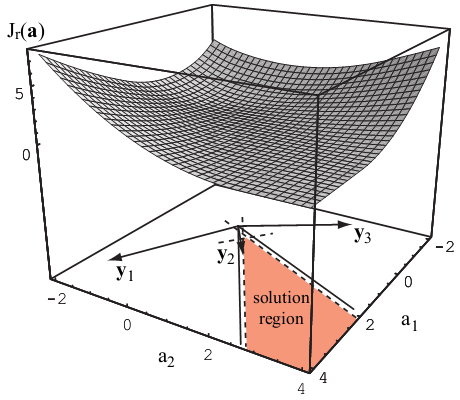
\includegraphics[width=6cm]{./images/relaxation.png}
    	 Criterion function of $\bm J_r(a)$ with margin $b$
    \end{minipage}
    
    \skriptsubsection{Nonseparable Behavior}{238}
    The algorithms up to now won't stop if the data is not separable. Moreover, we do not know if we get a ``good'' result if we stop after a long time.
    One way is to reduce the influence of the wrong classified sample with $\eta(k)=1/k$ so that the solution will end in a ``good'' area.
    
    \skriptsubsection{Minimum Squared-Error Procedures}{240}
    In comparison to the perceptron processes, here all samples are used. 
    The goal is to solve $\bm a^T \bm y_i = b_i$
    \begin{equation*}
    \bm Y \bm a = \bm b
    \qquad \text{or} \qquad
    \begin{bmatrix}
      y_{10} & y_{11} & \ldots & y_{1d}\\
      \vdots &\vdots & & \vdots\\
      \vdots &\vdots & & \vdots\\
      y_{n0} & y_{n1} & \ldots & y_{nd}\\
    \end{bmatrix}
    \begin{array}{c}
    \begin{bmatrix}
    	a_0\\
    	\vdots\\
    	a_d
    \end{bmatrix}\\
    \vphantom{\vdots}\\
    \end{array} = 
    \begin{bmatrix}
    	b_0\\
    	\vdots\\
    	\vdots\\
    	b_n
    \end{bmatrix} \qquad \text{with} \qquad n \gg d
    \end{equation*}
    
    where $\bm{b}$ is the \emph{margin vector} and $b_i$ have to be positive constants. 
    The criterion function $\bm J_S(\bm a)=\|\bm Y \bm a - \bm b \|^2$ lead 
    us to the minimum squared error (MSE) solution of $\bm Y \bm a = \bm b$
    \begin{equation*}
        \bm a = (\bm Y^T \bm Y)^{-1} \bm Y^T b = \bm Y^\dagger \bm b
    \end{equation*}
    where $\bm Y^\dagger \equiv (\bm Y^T \bm Y)^{-1} \bm Y^T$ is the \emph{pseudoinverse} of $\bm Y$.
    If $\bm Y$ is square and nonsingular, the pseudoinverse coincides with the regular inverse. \\

    Disadvantages of these algorithms are: High computational effort for computation of $\bm Y^\dagger$;
    possible singularities ($|\bm Y|$ close to zero); the separating vector is not necessarily found (see next figure);
    no clear abortion criterion (possibly: $|\eta(k) (\bm b - \bm a^T \bm y(k)) \bm y(k)| < \Theta$ with $\Theta$ being a threshold)\\
    
    \begin{wrapfigure}{r}{6cm}
        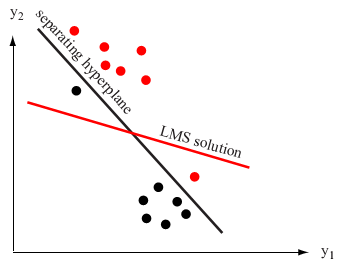
\includegraphics[width=6cm]{./images/LMS.png}
    \end{wrapfigure}
    
     As usual$\bm Y$ is built out of the augmented feature vector of $\omega_1$ and the augmented feature vector of $\omega_2$:\\
    $\bm Y = \begin{bmatrix}
    \bm 1_1 & \bm X_1 \\
    - \bm 1_2 & -\bm X_2  \\
    \end{bmatrix}$ \\
    
    \skriptsubsubsubsection{Algorithm: Widrow-Hoff / LMS Rule}{245}\\
    To avoid large matrix multiplications the LMS procedure updates the weight vector with every sample. 
    In contrast to the previous algorithms the LMS uses all samples.
    \begin{equation*}
        \bm a(k+1)=\bm a(k)+\eta(k)\left(\bm b-\bm a^T(k)\bm y(k)\right)\bm y(k)
    \end{equation*}
    
    $\eta(k)$ has to decrease with $k$ to obtain convergence, e.g. $\eta(k)=n(1)/k$\\

    \skriptsubsubsubsection{Fisher's Linear Discriminant}{242}\\
        With $\bm b=\begin{bmatrix}
        \frac{n}{n_1} \cdot \bm 1_1\\
        \frac{n}{n_2} \cdot \bm 1_2
        \end{bmatrix}$ the pseudoinverse minimizes the ratio between the intra scatter $\bm S_i$ and the
        scatter within two classes $\bm S_W = \sum_i \bm S_i$.\\
        
    \skriptsubsubsubsection{Asymptotic Approximation to an Optimal Discriminant}{243}\\
    With  $\bm b=\bm 1$ the pseudoinverse approximate to the Bayes discriminant function $g_0 = P(\omega_1 | \bm x) - P(\omega_2 | \bm x)$\\

 	\skriptsubsubsubsection{Stochastic Approximation Method}{247}\\
    The stochastic approximation method is an MSE procedure where the samples are drawn randomly.
    This results in a random sequence of weight vectors.
 	For each $\bm x$ we let $\theta$ be its \emph{label} with $\theta=+1$ if $\bm x$ is labeled $\omega_1$ and $\theta=-1$ if $\bm x$ is labeled $\omega_2$.
 	The label variable $\theta$ can be thought of as noisy version of the Bayes discriminant function $g_0(\bm x)$.
    This leads to the update rule
    \begin{equation*}
        \bm a(k+1)=a(k)+\eta(k)(\theta_k - \bm a^T(k)\bm y_k)\bm y_k
    \end{equation*}
  	which is basically just the Widrow-Hoff rule.
  	With $\eta(k)=1/k$ the convergence is often very slow.
  	A stochastic analog to \emph{Newton's rule} for would be
  	\begin{equation*}
     	\bm a(k+1)=a(k)+\bm R_{k+1}(\theta_k - \bm a^T(k)\bm y_k)\bm y_k
     	\quad \text{with} \quad 
     	\bm R_{k+1}^{-1}= \bm R_{k}^{-1} + \bm y_k \bm y_k^T
     	\quad \text{or} \quad
     	\bm R_{k+1}= \bm R_{k} + \frac{\bm R_{k} \bm y_k(\bm R_{k} \bm y_k)^T}{1+\bm y_k^T \bm R_{k} \bm y_k}
 	\end{equation*}
 	where $\bm R_{k}$ is the covariance matrix, which is updated every sample.
 	
 	
 	\skriptsubsection{Ho-Kashyap Procedures}{249}
 	The advantage of the \em Ho-Kashyap procedures \em is that the separating vector will be found in finite time, if the data is separable, or the 
 	solution will converge to the MSE solution in infinite time.
 	The idea is to adapt $\hat{\bm a}$ and $\hat{\bm b}$ in the MSE equation $\bm Y \hat{\bm a} = \hat{\bm b}$.
 	If the training samples are \textbf{lineary separable} a solution can be found so that 
 	\textbf{every component} $\hat{b_i}> 0$. Finally, $\bm e(k) = 0$ for a real solution or 
 	all $\bm e(k) \leq 0$ (all components not positive) when the samples are not linearly separable.\\
 	
 	\subsubsubsection{Descent Procedure}\\
 	The criterion function is the same as in LMS: $\bm J_S(\bm a)=\|\bm Y \bm a - \bm b \|^2$. 
 	But instead of updating only $\bm a$ vector $\bm b$ is also updated:
 	$$ \bm b(k+1)=\bm b(k)- \eta(k) \frac{1}{2} \left(\bm{\nabla_b J}_s - |\bm{\nabla_b J}_s|\right) \qquad 
 	0 <\eta < 2/\lambda_{max} \; (\lambda \text{ are the eigenvalues of } \bm Y^T \bm Y)$$
 	$|\bm{\nabla_b J}_s|$ states that every component is positive. 
 	Gradient of $\bm J$ by $b$: $\bm{\nabla_b J}_s = 2\bm Y^T(\underbrace{\bm{Y a - b}}_{=e})$
 	
 	The only problem is, that the procedure only stops if the data are linear separable and convergence 
 	is only achieved in \textbf{finite} steps. There is no boundary of steps and hence, \textbf{when should be stopped?}\\
 	 
 	 
 	\skriptsubsubsubsection{Modified Ho-Kashyap}{254}
 	  The modified Ho-Kashyap uses the property that $\bm Y^\dagger \bm e(k) = 0$ and brings the advantage
 	  that the expensive pseudoinverse $\bm Y^\dagger$ has to be calculated only once at the start. It
 	  modifies the update rules compared to the general Ho-Kashyap and is always to be preferred.
 	  
 	  \begin{tabular}{lll}
 	    Init 
 	      &$\bm b(1) > 0$ (arbitrary) 
 	      &$\bm a(1) = \bm Y^\dagger \bm b(1)$\\
 	    Update 
 	      &$\bm b(k+1) = \bm b(k) + \eta (\underbrace{\bm e(k) + |\bm e(k)|}_{2e^+})$ 
 	      &$\bm a(k+1) = \bm a(k) + \eta \bm Y^\dagger |\bm e(k)|$
    \end{tabular}
 	
 	\skriptsubsubsubsection{Related Procedures}{254}
 	  This approach avoids the computation of $\bm Y^\dagger$ by introducing a matrix $\bm R$. 
 	  
    \begin{tabular}{lll}
      Init 
        &$\bm b(1) > 0$ (arbitrary) 
        &$\bm a(1)$ (arbitrary)\\
      Update 
        &$\bm b(k+1) = \bm b(k) + \eta (\bm e(k) + |\bm e(k)|)$ 
        &$\bm a(k+1) = \bm a(k) + \eta \bm R \bm Y^T |\bm e(k)|$
    \end{tabular}
 	  
 	  When $\bm R = \bm 1$ the step size becomes $\eta(k) = \frac{\|\bm Y^T |e(k|)\|^2}{\|\bm Y \bm Y^T |e(k)|\|^2}$.\\
 	  When $\bm R = \frac{1}{\eta} (\bm Y^T \bm Y)^{-1}$ this procedure becomes the original Ho-Kashyap.
 	
 	\skriptsubsection{Support Vector Machines (SVM)}{259}
    % This section closely follows the lecture notes on support vector machines by Andrew Ng (http://cs229.stanford.edu/notes/cs229-notes3.pdf)
    %TODO: add nice image
    We define the \emph{functional margin} of the hyperplane $(w,b)$ to a training example $(x^{(i)},y^{(i)})$ by
    \begin{equation*}
        \hat{\lambda}^{(i)} = y^{(i)} (w^T x + b)
    \end{equation*}
    as multiplying $w$ and $b$ by a factor increases the functional margin without changing the separating hyperplane, 
    the \emph{geometric margin} to a training example is introduced by
    \begin{equation*}
        \lambda^{(i)} = y^{(i)} \left( \left( \frac{w}{||w||} \right)^T x^{(i)} + \frac{b}{||w||} \right)
    \end{equation*}
    
    The \emph{geometric margin} $\lambda$ is the smallest of the geometric margins of a training set $\lambda = \min\limits_{i=1,\ldots,m}\lambda^{(i)}$.
    
    \paragraph{Optimal margin classifier}~\\
    An optimal margin classifier can be achieved by maximizing $\lambda$ subject to $y^{(i)}(w^T x^{(i)}+b)\leq\lambda$ and $||w||=1$.
    This can be equivalently achieved by the following (primal) optimization problem
    \begin{equation*}
        \min_{w,b} \frac{1}{2} ||w||^2 \qquad \text{s.t.} \quad y^{(i)}(w^T x^{(i)} + b) \geq 1, \quad i=1,\ldots,m
    \end{equation*}
    which can be converted to the dual optimization problem
    \begin{equation*}
        \max_{\alpha} \sum\limits_{i=1}^m \alpha_i - \frac{1}{2}\sum\limits_{i,j=1}^m y^{(i)}y^{(j)}\alpha_i\alpha_j \langle x^{(i)},x^{(j)} \rangle
        \qquad \text{s.t.} \quad \alpha_i \geq 0, \quad i=1,\ldots,m \qquad \text{and} \quad \sum\limits_{i=1}^m \alpha_i y^{(i)}=0
    \end{equation*}
    
    \paragraph{Kernels}~\\
    Let $\Phi(x)$ denote a \emph{feature mapping} which maps the attributes to a higher-dimensional feature space.
    Since the optimal margin classifier depends solely on inner products $\langle x,z \rangle$, 
    these inner products can be replaced by $\langle \Phi(x),\Phi(z) \rangle$. 
    By specifying a \emph{Kernel} to be $K(x,z) = \Phi(x)^T \Phi(z)$ we can replace $\langle x,z \rangle$ by $K(x,z)$ and the algorithm will use the features $\Phi$.
    This allows the SVM to learn in a high-dimensional feature space given by $\Phi$ without having to explicitly find the vectors $\Phi(x)$. \\
    
    The most common Kernel function is the radial basis function or Gaussian kernel 
    $K(x,z) = \exp\left(-\frac{||x-z||^2}{2 \sigma^2}\right)$
    which corresponds to an infinite dimensional feature mapping $\Phi$.  \\
    
    \paragraph{Regularization and the non-separable case}~\\
    To make the algorithm work for non-linearly separable datasets as well as be less sensitive to outliers, we use $l_1$ regularization:
    \begin{equation*}
        \min_{w,b} \frac{1}{2}||w||^2 + C \sum\limits_{i=1}^m \xi_i
        \qquad \text{s.t.} \quad
        y^{(i)}(w^T x^{(i)} + b) \geq 1-\xi_i,
        \quad \text{and} \quad
        \xi_i \geq 0,
        \qquad i=1,\ldots,m
    \end{equation*}
    This allows functional margins less than 1, but increases the objective function by $C\xi_i$.
    The parameter $C$ controls the weighing between making $||w||^2$ small and ensuring that most examples have a margin of at least 1.
    The dual optimization problem is
    \begin{equation*}
        \max_{\alpha} \sum\limits_{i=1}^m \alpha_i - \frac{1}{2}\sum\limits_{i,j=1}^m y^{(i)} y^{(j)} \alpha_i \alpha_j \langle x^{(i)},x^{(j)} \rangle
        \qquad \text{s.t.} \quad
        0 \leq \alpha_i \leq C, \quad i=1,\ldots,m
        \qquad \text{and} \quad
        \sum\limits_{i=1}^m \alpha_i y^{(i)}=0
    \end{equation*}
    
    The Lagrangian multipliers $\alpha_i$ contain information on the corresponding training point:
    \begin{align*}
        \alpha_i = 0 & \quad\Rightarrow\quad y^{(i)}(w^T x^{(i)}+b) \geq 1 \qquad \text{training point is classified correctly}\\
        \alpha_i = C & \quad\Rightarrow\quad y^{(i)}(w^T x^{(i)}+b) \leq 1 \qquad \text{training point violates constraints}\\
        0 < \alpha_i < C & \quad\Rightarrow\quad y^{(i)}(w^T x^{(i)}+b) = 1 \qquad \text{training point is a support vector}\\
    \end{align*}
 	
 	\skriptsubsection{Overview over Different Procedures}{260} 
 	
 	\skriptsubsection{Multicategory Generalization}{265}
 	To handle \em multicategory cases \em with the \textbf{Kesler's Construction} the dimension of 
 	the weight vector $\bm a$ has to be extended by factor $c$
 	 and $(c-1)c$ new training samples generated:
 	$$ \bm{ \hat{a} }=\begin{bmatrix}
 	\bm a_1\\
 	\bm a_2\\
 	\vdots\\
 	\bm a_c
 	\end{bmatrix} \quad \text{and} \quad \bm \eta_{12}=\begin{bmatrix}
 	\bm y\\
 	-\bm y\\
 	\bm 0\\
 	\vdots\\
 	\bm 0
 	\end{bmatrix}; \quad \bm \eta_{13}=\begin{bmatrix}
 	\bm y\\
 	\bm 0\\
 	- \bm y\\
 	\vdots\\
 	\bm 0
 	\end{bmatrix}, \quad \ldots,\quad \bm \eta_{1c}=\begin{bmatrix}
 	\bm y\\
 	\bm 0\\
 	\bm 0\\
 	\vdots\\
 	-\bm y
 	\end{bmatrix}
 	$$
 	$c$ is the number of classes. Now the problem is again a two class problem. The solution solves the inequality:
 	$$\bm{\hat{a}}^T\bm \eta_{ji}>0$$
 	if the problem is linear separable. 
 	This idea is working for the most procedures except for the MSE or linear programming approaches (see \formelbuch{268}).
 	The fact that this needs many more samples is not practical but it allows us to convert many 
 	multi-category problems into two-category problems.
 	